\definecolor{Red}{RGB}{217,33,32}
\definecolor{Blue}{RGB}{63,96,174}
\definecolor{Duck}{RGB}{83,158,182}
\definecolor{Green}{RGB}{109,179,136}
\definecolor{Yellow}{RGB}{202,184,67}
\definecolor{Orange}{RGB}{231,133,50}
\definecolor{Purple}{RGB}{120,28,129}
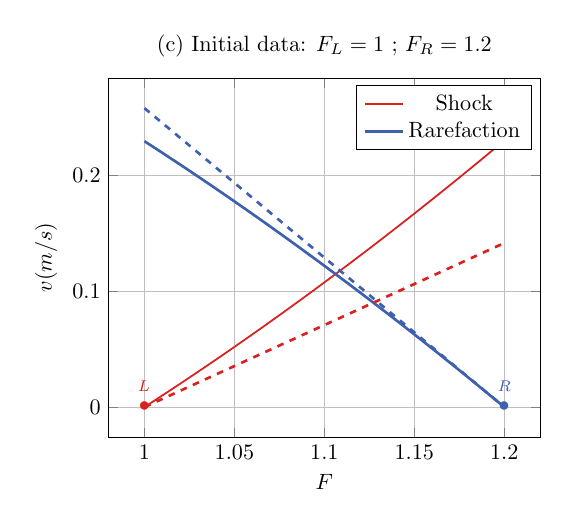
\begin{tikzpicture}[scale=0.8]
\begin{axis}[xlabel=$F$,ylabel=$v (m/s)$,ymajorgrids=true,xmajorgrids=true,title={(c) Initial data: $F_L=1$ ; $F_R=1.2$}]
\addplot[Red,thick] coordinates {(1.0,0.0) (1.003920392039204,0.003931917267080632) (1.0078407840784078,0.007886877524091035) (1.0117611761176117,0.011864869670167599) (1.0156815681568157,0.01586588273338493) (1.0196019601960196,0.019889905868838792) (1.0235223522352235,0.023936928356764118) (1.0274427442744274,0.028006939600686957) (1.0313631363136313,0.03209992912561001) (1.0352835283528352,0.0362158865762309) (1.0392039203920391,0.04035480171519238) (1.043124312431243,0.04451666442136419) (1.047044704470447,0.04870146468815503) (1.0509650965096509,0.0529091926218551) (1.0548854885488548,0.05713983844000771) (1.0588058805880587,0.06139339246981002) (1.0627262726272626,0.06566984514654124) (1.0666466646664667,0.06996918701201955) (1.0705670567056704,0.07429140871308397) (1.0744874487448746,0.07863650100010654) (1.0784078407840785,0.08300445472552491) (1.0823282328232824,0.08739526084240548) (1.0862486248624863,0.09180891040302837) (1.0901690169016902,0.09624539455749745) (1.0940894089408941,0.1007047045523746) (1.098009800980098,0.1051868317293367) (1.101930193019302,0.10969176752385594) (1.1058505850585059,0.11421950346390249) (1.1097709770977098,0.11877003116866883) (1.1136913691369137,0.12334334234731587) (1.1176117611761176,0.1279394287977403) (1.1215321532153215,0.13255828240536205) (1.1254525452545254,0.1371998951419326) (1.1293729372937293,0.14186425906436276) (1.1332933293329333,0.14655136631357016) (1.1372137213721372,0.1512612091133456) (1.141134113411341,0.15599377976923837) (1.145054505450545,0.16074907066745941) (1.148974897489749,0.1655270742738032) (1.1528952895289528,0.17032778313258656) (1.1568156815681567,0.17515118986560513) (1.1607360736073606,0.17999728717110672) (1.1646564656465646,0.18486606782278137) (1.1685768576857685,0.18975752466876733) (1.1724972497249724,0.19467165063067376) (1.1764176417641763,0.19960843870261824) (1.1803380338033802,0.20456788195028056) (1.1842584258425841,0.20954997350997065) (1.188178817881788,0.21455470658771253) (1.192099209920992,0.21958207445834133) (1.196019601960196,0.2246320704646163) (1.1999399939993998,0.229704688016345) };
\addplot[Blue,very thick] coordinates {(1.0,0.22917941198468886) (1.003920392039204,0.2252475003389243) (1.0078407840784078,0.22129257921328083) (1.0117611761176117,0.21731469262755104) (1.0156815681568157,0.21331388384346875) (1.0196019601960196,0.20929019538339458) (1.0235223522352235,0.20524366904839547) (1.0274427442744274,0.20117434593574032) (1.0313631363136313,0.19708226645583485) (1.0352835283528352,0.19296747034862255) (1.0392039203920391,0.18882999669946615) (1.043124312431243,0.184669883954535) (1.047044704470447,0.1804871699357172) (1.0509650965096509,0.1762818918550712) (1.0548854885488548,0.17205408632883865) (1.0588058805880587,0.1678037893910336) (1.0627262726272626,0.16353103650662262) (1.0666466646664667,0.15923586258431413) (1.0705670567056704,0.1549183019889692) (1.0744874487448746,0.15057838855364641) (1.0784078407840785,0.1462161555913001) (1.0823282328232824,0.14183163590613646) (1.0862486248624863,0.13742486180464666) (1.0901690169016902,0.1329958651063243) (1.0940894089408941,0.12854467715408055) (1.098009800980098,0.12407132882436642) (1.101930193019302,0.11957585053701415) (1.1058505850585059,0.11505827226480363) (1.1097709770977098,0.11051862354276928) (1.1136913691369137,0.10595693347725012) (1.1176117611761176,0.10137323075469579) (1.1215321532153215,0.09676754365023553) (1.1254525452545254,0.09213990003601796) (1.1293729372937293,0.08749032738932871) (1.1332933293329333,0.08281885280049482) (1.1372137213721372,0.07812550298058156) (1.141134113411341,0.07341030426888846) (1.145054505450545,0.0686732826402522) (1.148974897489749,0.06391446371216106) (1.1528952895289528,0.05913387275168875) (1.1568156815681567,0.05433153468225065) (1.1607360736073606,0.04950747409019151) (1.1646564656465646,0.04466171523120707) (1.1685768576857685,0.03979428203660571) (1.1724972497249724,0.03490519811941557) (1.1764176417641763,0.029994486780341414) (1.1803380338033802,0.025062171013576353) (1.1842584258425841,0.020108273512470697) (1.188178817881788,0.015132816675066284) (1.192099209920992,0.010135822609495795) (1.196019601960196,0.0051173131392549635) (1.1999399939993998,7.730980834955399e-05) };
\legend{Shock,Rarefaction}
\node at (axis cs:1,0) [Red] {$\bullet$};
  \node at (axis cs:1.2,0) [Blue] {$\bullet$};
  \node at (axis cs:1,0) [anchor=south,Red] {$\Qcb^L$};
  \node at (axis cs:1.192,0) [above right,Blue] {$\Qcb^R$};
  \addplot[Blue,dashed,very thick,domain=1:1.2,samples=51,samples y=0]
    ({x},{0.-sqrt(0.5*(3.*(1.2^2)-1))*(x-1.2)});
  \addplot[Red,dashed,very thick,domain=1:1.2,samples=51,samples y=0]
  ({x},{0.+sqrt(0.5*(2.-1))*(x-1.)});
\legend{Shock,Rarefaction}
\end{axis}
\end{tikzpicture}
